%%%%%%%%%%%%%%%%%%%%%%%%%%%%%%%%%%%%%%%%%%%%%%%%%%%%%%%%%%%%%%%%%%%%%%%%%%%

\documentclass[a4paper,oneside,12pt]{article}
\usepackage{mystyle}

\begin{document}

\title{\Large\bf Linear functions}
\author{%%
  Minh Van Nguyen \\
  \url{mvngu@gmx.com}
}
\date{\today}
\maketitle

\begin{packeditem}
\item Application of linear equations: fill a bucket with water.
\end{packeditem}

%%%%%%%%%%%%%%%%%%%%%%%%%%%%%%%%%%%%%%%%%%%%%%%%%%%%%%%%%%%%%%%%%%%%%%%%%%%

\section{General form}
\label{sec:general_form}

A \emph{linear function} is an expression of the form
%%
\begin{equation}
\label{eqn:linear_function_general}
f(x)
=
ax + b.
\end{equation}
%%
The numbers $a$ and $b$ are fixed real numbers, while $x$ is a
variable that can be any real number.  What does the function $f(x)$
look like?

As an example, set $a = b = 1$ so that you have $f(x) = x + 1$.  The
graph of $f(x) = x + 1$ is a straight line that passes through the
point $A = \tuple{-1}{0}$ on the $x$-axis and the point
$B = \tuple{0}{1}$ on the $y$-axis.  How were the coordinates of $A$
and $B$ calculated?  For the point $A$, you set $f(x) = 0$ and solve
the equation $0 = x + 1$ for $x$ to get $x = -1$.  The $x$-coordinate
of $A$ is $-1$ and the $y$-coordinate is $0$.  For the point $B$,
you set $x = 0$ and solve the equation $y = 0 + 1$ for $y$ to obtain
$y = 1$.  Then $B$ has $x$-coordinate $0$ and $y$-coordinate $1$.  You
plot the points $A$ and $B$, then draw a straight line through those
two points to produce the graph in \Figure{fig:plot_x_+_1}.

\begin{figure}[!htbp]
\centering
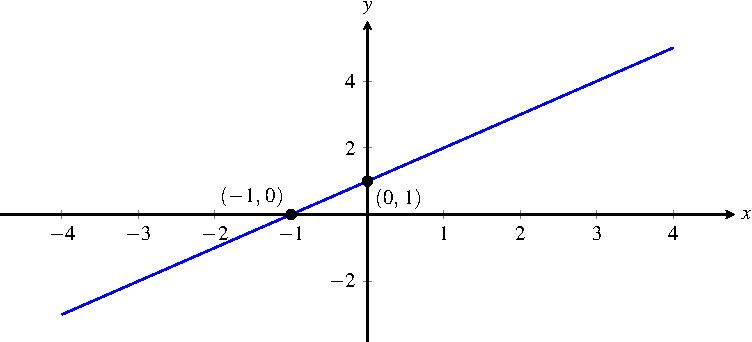
\includegraphics[scale=1]{image/06/a-1-b-1.pdf}
\caption{%%
  A graph of the function $f(x) = x + 1$.
}
\label{fig:plot_x_+_1}
\end{figure}

In general, how would you draw the graph of the
\Function{eqn:linear_function_general}?  As in the example above, you
want to determine two different points of the function $f(x)$.  A
common way to do so is as follows.  You set $f(x) = 0$ and determine
the point $A = \tuple{\alpha}{0}$, where $x = \alpha$ is obtained by
solving $f(x) = 0$ for $x$.  You then set $x = 0$ and determine the
point $B = \tuple{0}{\beta}$, where $\beta = f(0)$.  Plot the points
$A$ and $B$, then draw a straight line through those two points.  The
result is a graph of the \Function{eqn:linear_function_general}.
Let's put the above strategy into practice.

Suppose in \Equation{eqn:linear_function_general} you set $a = 2$ and
$b = -1 / 2$.  How would you draw a graph of the function
$f(x) = 2x - \frac{1}{2}$?  To obtain the point $A$, you set
$f(x) = 0$ and solve the equation $0 = 2x - \frac{1}{2}$ for $x$.  The
latter equation can be written as $2x = \frac{1}{2}$ and dividing both
sides by $2$ shows that
%%
\begin{align*}
x
&=
\frac{1}{2} \div 2 \\[4pt]
&=
\frac{1}{2} \times \frac{1}{2} \\[4pt]
&=
\frac{1}{4}.
\end{align*}
%%
So you have $A = \tuple{\frac{1}{4}}{0}$.  The coordinates of the
point $B$ are determined by first setting $x = 0$.  You then solve the
equation $y = 2 \times 0 - \frac{1}{2}$ for $y$.  The latter equation
can be written as
%%
\begin{align*}
y
&=
2 \times 0 - \frac{1}{2} \\[4pt]
&=
0 - \frac{1}{2} \\[4pt]
&=
-\frac{1}{2}
\end{align*}
%%
and you have $B = \tuple{0}{-\frac{1}{2}}$.  Plot the points $A$ and
$B$ and draw a straight line through the two points to produce the
graph in \Figure{fig:plot_2x_minus_half}.

\begin{figure}[!htbp]
\centering
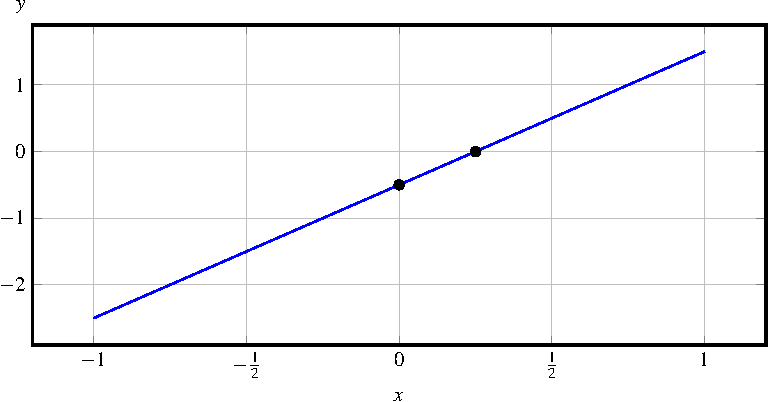
\includegraphics[scale=1]{image/06/a-2-b-minus-half.pdf}
\caption{%%
  A graph of the function $f(x) = 2x - \frac{1}{2}$.
}
\label{fig:plot_2x_minus_half}
\end{figure}

\begin{exercise}
Draw a graph of the function $f(x) = 2x - 2$.
\end{exercise}

\ifbool{showSolution}{
\begin{solution}
You want two different points $A$ and $B$ of the function
$f(x) = 2x - 2$.  A graph of the function is obtained by drawing a
straight line through those two points.  First, you set $f(x) = 0$ and
solve the equation $0 = 2x - 2$ for $x$.  You can write the latter
equation as $2x = 2$ and dividing both sides by $2$ shows that
$x = 1$.  Thus you have the point $A = \tuple{1}{0}$.  Second, you set
$x = 0$ and solve the equation $y = 2 \times 0 - 2$ for $y$.  Write
the last equation as $y = 0 - 2$ and you see that $y = -2$.  Thus you
have the point $B = \tuple{0}{-2}$.  Plot the two points $A$ and $B$,
draw a straight line through those two points, and you have the graph
in \Figure{fig:plot_2x_minus_2}.

\begin{figure}[!htbp]
\centering
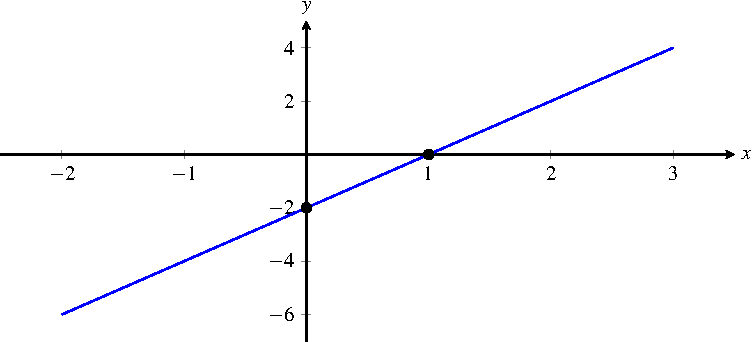
\includegraphics[scale=1]{image/06/a-2-b-minus-2.pdf}
\caption{%%
  A graph of the function $f(x) = 2x - 2$.
}
\label{fig:plot_2x_minus_2}
\end{figure}
\end{solution}
}{}

\begin{exercise}
Draw a graph of the function $f(x) = 3x + \frac{1}{2}$.
\end{exercise}

\ifbool{showSolution}{
\begin{solution}
Determine two points of the function $f(x)$ and draw a straight line
through those two points to produce a graph of the function.  For the
first point, set $f(x) = 0$ and solve the equation
$0 = 3x + \frac{1}{2}$ for $x$.  The latter equation can be written as
$3x = -\frac{1}{2}$.  Multiply both sides by $\frac{1}{3}$ to see that
$x = -\frac{1}{2} \times \frac{1}{3} = -1 / 6$ and you have the point
$A = \tuple{-\frac{1}{6}}{0}$.  For the second point, set $x = 0$ and
solve the equation $y = 3 \times 0 + \frac{1}{2}$ for $y$.  The last
equation can be written as $y = 1 / 2$ and you have the point
$B = \tuple{0}{\frac{1}{2}}$.  Plot the two points and draw a straight
line through those two points to produce the graph in
\Figure{fig:plot_3x_half}.

\begin{figure}[!htbp]
\centering
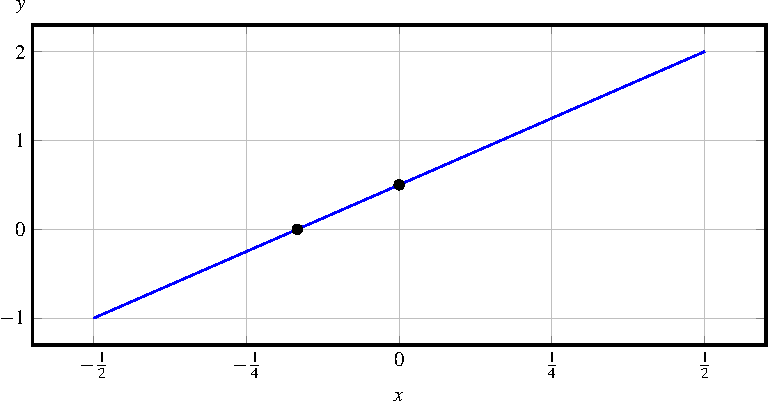
\includegraphics[scale=1]{image/06/a-3-b-half.pdf}
\caption{%%
  A graph of the function $f(x) = 3x + \frac{1}{2}$.
}
\label{fig:plot_3x_half}
\end{figure}
\end{solution}
}{}


%%%%%%%%%%%%%%%%%%%%%%%%%%%%%%%%%%%%%%%%%%%%%%%%%%%%%%%%%%%%%%%%%%%%%%%%%%%

\section{Special cases}

Consider the case where $a = 0$ in
\Equation{eqn:linear_function_general}.  Then you have $f(x) = b$,
which states that no matter what the value of $x$ is you will always
get $y = b$.  For this reason, the function $f(x) = b$ is called a
\emph{constant function}.  The graph of the constant function
$f(x) = b$ is a horizontal line through the point $b$ on the
$y$-axis and this horizontal line is parallel to the $x$-axis.  See
\Figure{fig:constant_functions} for the examples of $b = 2$ and
$b = -3$.

\begin{figure}[!htbp]
\centering
\subfigure[]{
  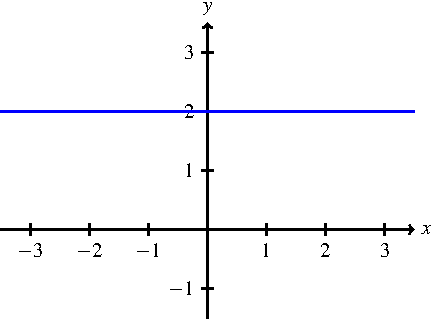
\includegraphics[scale=0.8]{image/06/a-0-b-2.pdf}
}
%%
\qquad
%%
\subfigure[]{
  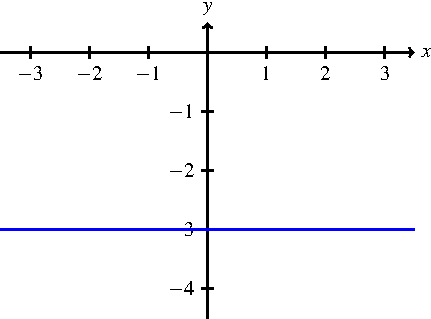
\includegraphics[scale=0.8]{image/06/a-0-b-minus-3.pdf}
}
\caption{%%
  Plots of the constant functions (a)~$f(x) = 2$ and
  (b)~$f(x) = -3$.
}
\label{fig:constant_functions}
\end{figure}

\begin{exercise}
Describe the function $f(x) = -1/2$ and draw its graph.
\end{exercise}

\ifbool{showSolution}{
\begin{solution}
The expression $f(x) = -1/2$ is a constant function.  Its graph is a
horizontal line through the point $-1/2$ on the $y$-axis and this line
is parallel to the $x$-axis.
\Figure{fig:constant_function_minus_half} shows a graph of the
function $f(x)$.
%%
\begin{figure}[!htbp]
\centering
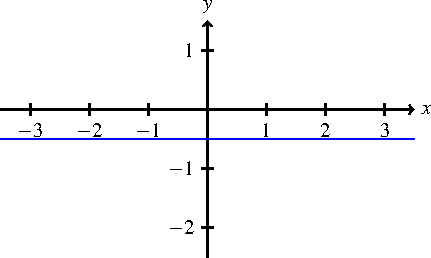
\includegraphics[scale=1]{image/06/a-0-b-minus-half.pdf}
\caption{%%
  A graph of the constant function $f(x) = -1/2$.
}
\label{fig:constant_function_minus_half}
\end{figure}
\end{solution}
}{}

\begin{exercise}
\label{ex:constant_function_zero}
Describe the graph of the expression $f(x) = 0$.
\end{exercise}

\ifbool{showSolution}{
\begin{solution}
The expression $f(x) = 0$ is a constant function whose graph is a
horizontal line through the point $0$ on the $y$-axis.  In other
words, the function $f(x) = 0$ describes the $x$-axis.
\end{solution}
}{}

Now consider the case of $b = 0$ in
\Equation{eqn:linear_function_general} so that you have
$f(x) = ax$.  If you also have $a = 0$, then $f(x)$ is reduced to the
function in \Exercise{ex:constant_function_zero}.  Otherwise assume
that $a \neq 0$.  What does the graph of $f(x) = ax$ look like?

Let's use the strategy from \Section{sec:general_form} to graph
$f(x) = ax$.  Set $f(x) = 0$ and solving the equation $0 = ax$ for $x$
results in $x = 0$.  You have the point $A = \tuple{0}{0}$.  Next, set
$x = 0$ and solving the equation $y = a \times 0$ for $y$ shows that
$y = 0$.  You also have the point $B = \tuple{0}{0}$.  Both of $A$ and
$B$ are the same point and that point is the origin.  You need another
way to determine a second and different point of the function
$f(x) = ax$.

Instead of setting $x = 0$, you can try setting $x = 1$.  Simplify the
equation $y = a \times 1$ and you obtain $y = a$.  Hence the
second~(and different) point is $\tuple{1}{a}$.  In other words, if
$a \neq 0$ then the graph of $f(x) = ax$ is a straight line that
passes through the origin.  \Figure{fig:function_ax_positive_rational}
shows some graphs of $f(x) = ax$, where $a$ is a positive real number
that is at most $1$, i.e.~$0 < a \leq 1$.
\Figure{fig:function_ax_positive_at_least_one} shows some graphs of
$f(x) = ax$ for the case where $a \geq 1$.  Notice that in both of
these figures, the graphs of $f(x) = ax$ pass through the point
$\tuple{0}{0}$.

\begin{figure}[!htbp]
\centering
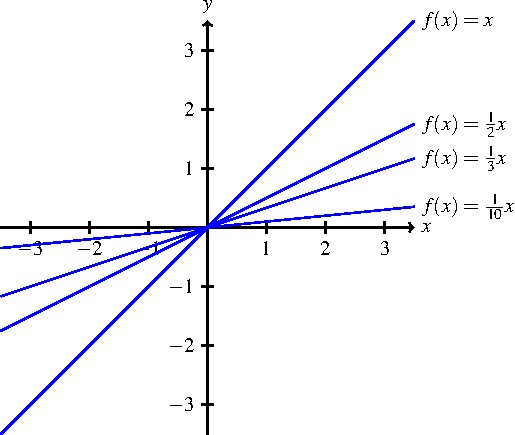
\includegraphics[scale=1]{image/06/ax-small.pdf}
\caption{%%
  Graphs of the function $f(x) = ax$ for various values of $a$, where
  it is assumed that $0 < a \leq 1$.  As the value of $a$ becomes
  smaller and smaller, the graph of $f(x) = ax$ becomes more and more
  like a horizontal line.
}
\label{fig:function_ax_positive_rational}
\end{figure}

\begin{figure}[!htbp]
\centering
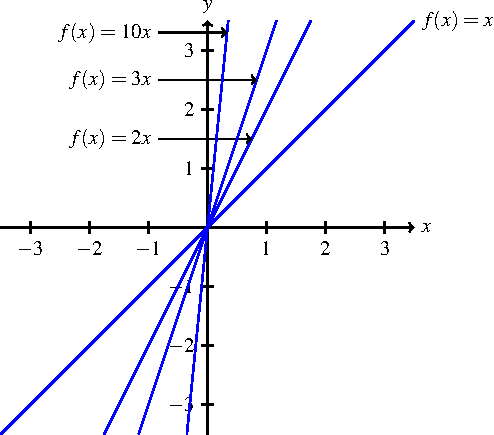
\includegraphics[scale=1]{image/06/ax-large.pdf}
\caption{%%
  Graphs of the function $f(x) = ax$ for various values of $a$, where
  $a \geq 1$.  As the value of $a$ becomes larger and larger, the
  graph of $f(x) = ax$ becomes steeper and steeper like a vertical
  line.
}
\label{fig:function_ax_positive_at_least_one}
\end{figure}

\begin{exercise}
Describe the graphs of the function $f(x) = ax$, where the factor $a$
takes on the values
$a = \quadruple{-\frac{1}{10}}{-\frac{1}{3}}{-\frac{1}{2}}{-1}$.
\end{exercise}

\ifbool{showSolution}{
\begin{solution}
\Figure{fig:graph_ax_a_negative_between_0_minus_1} shows the graphs of
$f(x) = ax$ for the above given values of $a$.  Note that
$-1 \leq a < 0$.  As $a$ becomes larger and larger and approches zero,
the graph of $f(x) = ax$ becomes more and more like a horizontal line.

\begin{figure}[!htbp]
\centering
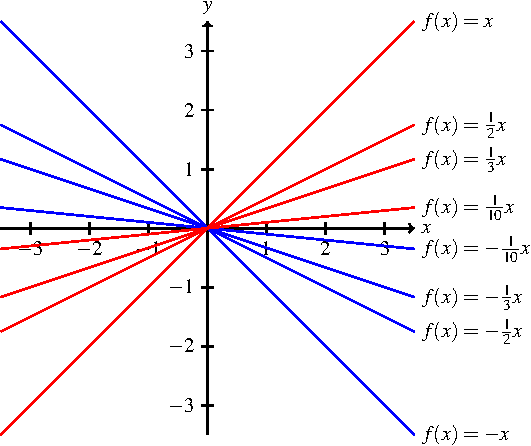
\includegraphics[scale=1]{image/06/ax-small-negative.pdf}
\caption{%%
  The blue lines are graphs of the function $f(x) = ax$, where $a$ has
  the values
  $a = \quadruple{-\frac{1}{10}}{-\frac{1}{3}}{-\frac{1}{2}}{-1}$.
  The red lines are reflections about the $x$-axis of the blue lines.
}
\label{fig:graph_ax_a_negative_between_0_minus_1}
\end{figure}
\end{solution}
}{}

\begin{exercise}
Describe the graphs of the function $f(x) = ax$, where the factor $a$
takes on the values $a = \quadruple{-1}{-2}{-3}{-10}$.
\end{exercise}

\ifbool{showSolution}{
\begin{solution}
\Figure{fig:graph_ax_a_negative_less_than_1} shows the graphs of
$f(x) = ax$ for the above given values of $a$.  Starting from
$a = -1$, as $a$ becomes smaller and smaller, the graph of
$f(x) = ax$ becomes steeper and steeper like a vertical line.

\begin{figure}[!htbp]
\centering
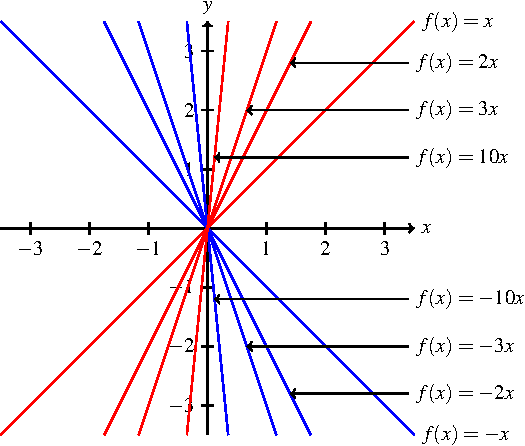
\includegraphics[scale=1]{image/06/ax-large-negative.pdf}
\caption{%%
  The blue lines are graphs of the function $f(x) = ax$, where $a$ has
  the values $a = \quadruple{-1}{-2}{-3}{-10}$.  The red lines are
  reflections about the $x$-axis of the blue lines.
}
\label{fig:graph_ax_a_negative_less_than_1}
\end{figure}
\end{solution}
}{}

\end{document}
